\documentclass[12pt]{article}

\usepackage{fullpage}
\usepackage{graphicx}
\usepackage{amssymb}
\usepackage{amsmath}
\usepackage[none]{hyphenat}
\usepackage{parskip}
\usepackage[spanish]{babel}
\usepackage[utf8]{inputenc}
\usepackage{hyperref}
\usepackage{fancyhdr}
\usepackage{tasks}
\usepackage{mdframed}
\usepackage{xcolor}
\usepackage{pgfplots}
\usepackage[makeroom]{cancel}
\usepackage{multicol}
\usepackage[shortlabels]{enumitem}
\usepackage{stackrel}
\usepackage{tkz-tab}
\usepackage{xpatch}
\usepackage{tkz-euclide}
\usetkzobj{all}
\xpatchcmd{\tkzTabLine}{$0$}{$\bullet$}{}{}

\setlength{\headheight}{10pt}
\setlength{\headsep}{10pt}
\pagestyle{fancy}
\rhead{\ayudantia \ - \alumno}
\tikzset{t style/.style={style=solid}}

\newcommand*{\mybox}[2]{\colorbox{#1!30}{\parbox{.98\linewidth}{#2}}}

\newenvironment{solucion}
{\begin{mdframed}[backgroundcolor=black!10]
		{\bf Solución:}\\
	}
	{
	\end{mdframed}
}

\newenvironment{alternativas}[1]
{\begin{multicols}{#1}
		\begin{enumerate}[a)]
		}
		{
		\end{enumerate}
	\end{multicols}
}

\newenvironment{preguntas}
{\begin{enumerate}\itemsep12pt
	}
	{
	\end{enumerate}
}

\newcommand{\ayudantia}{{\sc Ayudantía 3.5}}
\newcommand{\tituloayu}{Compilado I1}
\newcommand{\fecha}{28 de agosto de 2019}
\newcommand{\sigla}{MAT1620}
\newcommand{\nombre}{Cálculo II}
\newcommand{\profesor}{Wolfgang Rivera}
\newcommand{\ano}{2019}
\newcommand{\semestre}{2}
\newcommand{\mail}{mat1620@ifcastaneda.cl}
\newcommand{\alumno}{Ignacio Castañeda - \mail}

\newcommand{\ev}{\Big|}
\newcommand{\ra}{\rightarrow}
\newcommand{\lra}{\leftrightarrow}
\newcommand{\N}{\mathbb{N}}
\newcommand{\R}{\mathbb{R}}
\newcommand{\Exp}[1]{\mathcal{E}_{#1}}
\newcommand{\List}[1]{\mathcal{L}_{#1}}
\newcommand{\EN}{\Exp{\N}}
\newcommand{\LN}{\List{\N}}
\newcommand{\comment}[1]{}
\newcommand{\lb}{\\~\\}
\newcommand{\eop}{_{\square}}
\newcommand{\hsig}{\hat{\sigma}}
\newcommand{\widesim}[2][1.5]{
	\mathrel{\overset{#2}{\scalebox{#1}[1]{$\sim$}}}
}
\newcommand{\wsim}{\widesim{}}
\newcommand{\lh}{\stackrel{L'H}{=}}

\begin{document}
\thispagestyle{empty}

\begin{minipage}{2cm}
	
\includegraphics[width=2cm]{../../../../img/logo.pdf}
	\vspace{0.5cm}
\end{minipage}
\begin{minipage}{\linewidth}
	\begin{tabular}{lrl}
		{\scriptsize\sc Pontificia Universidad Catolica de Chile} & \hspace*{0.7in}Curso: &
		\sigla  - \nombre\\
		{\sc Facultad de Matemáticas}&
		Profesor: & \profesor \\
		{\sc Semestre \ano-\semestre} & Ayudante: & {Ignacio Castañeda}\\
		& {Mail:} & \texttt{\mail}
	\end{tabular}
\end{minipage}

\vspace{-10mm}
\begin{center}
	{\LARGE\bf \ayudantia}\\
	\vspace{0.1cm}
	{\tituloayu}\\
	\vspace{0.1cm}
	\fecha\\
	\vspace{0.4cm}
\end{center}

\begin{preguntas}
\item Determinar si las siguientes integrales impropias convergen o divergen y calcularlas en caso de que converjan.
\begin{tasks}(3)
\task $\displaystyle\int_{0}^{3}\dfrac{1}{x\ \sqrt[]{x}}dx$
\task $\displaystyle\int_{e}^{\infty}\dfrac{1}{xlnx}dx$
\task $\displaystyle\int_{0}^{\infty}\dfrac{1}{\sqrt[]{x}(1+x)}dx$
\end{tasks}
\begin{solucion}

\begin{enumerate}[a)]
\item $\displaystyle\int_{0}^{3}\dfrac{1}{x\ \sqrt[]{x}}dx
			= \lim\limits_{z\ra 0} \displaystyle\int_{z}^{3}\dfrac{1}{x^{3/2}}dx 
			= \lim\limits_{z\ra 0} \dfrac{x^{-1/2}}{-\dfrac{1}{2}}\ev_z^3 
			= \lim\limits_{z\ra 0} -2x^{-1/2} \ev_z^3$\\
			$= \lim\limits_{z\ra 0} -2(3^{-1/2}-z^{-1/2})
			 = -2\left(\dfrac{1}{3^{1/2}} - \cancelto{\infty}{\dfrac{1}{z^{1/2}}}\right) = \infty = \not \exists$\\
			Luego, la integral diverge.
\item $\displaystyle\int_{e}^{\infty}\dfrac{1}{xlnx}dx$\\
			\\
			Usamos la sustitución $u=ln(x) \ra du = \dfrac{dx}{x}$,
			$$\displaystyle\int_{e}^{\infty}\dfrac{1}{xlnx}dx
			= \lim\limits_{a\ra \infty} \int_1^{ln(a)} \dfrac{du}{u}
			= \lim\limits_{a\ra \infty} ln(u) \ev_1^{ln(a)}
			= \lim\limits_{a\ra \infty} ln(ln(a)) - ln(1)$$
			$$= ln(ln(\infty)) = ln(\infty) = \infty = \not \exists$$
			Con lo que concluimos que la integral diverge
\item $\displaystyle\int_{0}^{\infty}\dfrac{1}{\sqrt[]{x}(1+x)}dx$\\
			\\
			Notemos que hay problemas en ambos límites de integración, por lo que debemos separar la integral en dos,
			$$\displaystyle\int_{0}^{\infty}\dfrac{1}{\sqrt[]{x}(1+x)}dx = \displaystyle\int_{0}^{1}\dfrac{1}{\sqrt[]{x}(1+x)}dx + \displaystyle\int_{1}^{\infty}\dfrac{1}{\sqrt[]{x}(1+x)}dx$$
			Calculemos primero la integral indefinida
			$$\displaystyle\int \dfrac{1}{\sqrt[]{x}(1+x)}dx$$
			Usando $u = \sqrt[]{x} \ra \dfrac{dx}{2\ \sqrt[]{x}}$,
			$$\int \dfrac{2du}{1+u^2} = 2\int \dfrac{du}{1+u^2} = 2arctan(u) = 2arctan(\sqrt[]{x})$$
			Luego,
			$$\displaystyle\int_{0}^{1}\dfrac{1}{\sqrt[]{x}(1+x)}dx + \displaystyle\int_{1}^{\infty}\dfrac{1}{\sqrt[]{x}(1+x)}dx$$
			$$= \lim\limits_{a\ra 0} 2arctan(\sqrt[]{x}) \ev_a^1 + \lim\limits_{a\ra \infty} 2arctan(\sqrt[]{x}) \ev_1^a$$
			$$= \lim\limits_{a\ra 0} 2(arctan(1) -arctan(\sqrt[]{a}))  + \lim\limits_{a\ra \infty} 2(arctan(\sqrt[]{a}) - arctan(1)) \ev_1^a$$
			$$= 2\left(\dfrac{\pi}{4} - 0\right) + 2\left(\dfrac{\pi}{2} - \dfrac{\pi}{4}\right)$$
			$$= \pi$$
			Por lo que la integral converge a $\pi$.
\end{enumerate}
\end{solucion}
\item La Trompeta de Torricelli se consigue al rotar la curva $y=\dfrac{1}{x},\ x \geq 1$ en torno al eje $x$.
\begin{enumerate}[a)]
\item Calcular la superficie de la trompeta entre $1$ y $L$ con la siguiente formula:
		$$ S = 2\pi \displaystyle\int_{1}^{L} f(x)\ \sqrt[]{1+[f'(x)]^2}dx, \quad con\ L \ra \infty $$
\item Calcular el volumen de la trompeta entre $1$ y $L$ con la siguiente formula:
		$$ V = \pi \displaystyle\int_{1}^{L} f(x)^2dx, \quad con\ L \ra \infty$$
\end{enumerate}
\begin{solucion}
En primer lugar,
			$$f(x) = \dfrac{1}{x} \ra f'(x) = -\dfrac{1}{x^2}$$
\begin{enumerate}[a)]
\item Calcular la superficie de la trompeta entre $1$ y $L$ con la siguiente formula:
			$$ S = 2\pi \displaystyle\int_{1}^{L} f(x)\ \sqrt[]{1+[f'(x)]^2}dx, \quad con\ L \ra \infty$$
			Usando la fórmula que nos dan,
			$$S = 2\pi \displaystyle\int_{1}^{\infty} \dfrac{1}{x}\ \sqrt[]{1+\left(-\dfrac{1}{x^2}\right)^2}dx 
			= 2\pi \displaystyle\int_{1}^{\infty} \dfrac{\sqrt[]{1+\frac{1}{x^4}}}{x}dx$$
			Notemos que
			$$\lim\limits_{x \ra \infty} \dfrac{\sqrt[]{1+\frac{1}{x^4}}}{x} = 
\lim\limits_{x \ra \infty} \dfrac{\sqrt[]{1+\cancelto{0}{\frac{1}{x^4}}}}{x} = 
\lim\limits_{x \ra \infty} \dfrac{1}{x} = 0$$
			Luego, usando $g(x) = \dfrac{1}{x}$, se cumple que
$$\lim\limits_{x \ra \infty} \dfrac{\dfrac{\sqrt[]{1+\frac{1}{x^4}}}{x}}{\dfrac{1}{x}} = 
\dfrac{\dfrac{1}{x}}{\dfrac{1}{x}} = 1 \neq 0$$
Por criterio de comparación al límite, $\displaystyle\int_{1}^{\infty} \dfrac{\sqrt[]{1+\frac{1}{x^4}}}{x}dx$ se comportará igual a $\displaystyle\int_{1}^{\infty} \dfrac{1}{x}dx$. Notemos que esta última diverge por criterio-p, ya que $p=1$.
			Finalmente,
			$$S = \infty$$
\item Calcular el volumen de la trompeta entre $1$ y $L$ con la siguiente formula:
			$$ V = \pi \displaystyle\int_{1}^{L} f(x)^2dx, \quad con\ L \ra \infty$$
			Usando la fórmula dada,
			$$V = \pi \displaystyle\int_{1}^{\infty} \left(\dfrac{1}{x}\right)^2dx
			=  \pi \displaystyle\int_{1}^{\infty} \dfrac{1}{x^2}dx
			= \pi \left(-\dfrac{1}{x}\ev_1^{\infty}\right)$$
			$$V = \pi$$
\end{enumerate}
\end{solucion}
\item Determinar el valor de la constante $C$ para la cual la integral
	$$\displaystyle\int_{0}^{\infty} \left( \dfrac{x}{x^2+1} - \dfrac{C}{3x+1}\right)dx$$
	converge. Evalúe la integral para este valor de $C$.
\begin{solucion}
Como habrán notado, al igual que los límites al infinito, en algunas integrales impropias podemos predecir si estas convergeran o divergeran por la diferencia de grados entre el numerador y el denominador. De esta forma, una integral como $\displaystyle\int_1^{\infty} \dfrac{x^2+1}{x^4}dx$ tendría la misma convergencia que $\displaystyle\int_1^{\infty} \dfrac{1}{x^2}dx$, ya que su diferencia de grados es 2. Esta última sabemos que converge, ya que es una integral $p$ con $p>1$. Vamos ahora al problema.\\
		\\
		En primer lugar, para ver como se comporta esta integral, juntemosla en una sola,
		\small$$\displaystyle\int_{0}^{\infty} \left( \dfrac{x}{x^2+1} - \dfrac{C}{3x+1}\right)dx
		= \displaystyle\int_{0}^{\infty} \dfrac{3x^2+x-Cx^2-C}{(x^2+1)(3x+1)}dx
		= \displaystyle\int_{0}^{\infty} \dfrac{x^2(3-C) + x - C}{(x^2+1)(3x+1)}dx$$
		Podemos ver que la diferencia de grado es $1$, por lo que se comportará igual a una integral $p$ con $p=1$, la cual diverge. Sin embargo, si $C=3$, el término $x^2$ se anula y la diferencia de grados es $2$, por lo que se comportará como la integral $p$ con $p=2>1$, la cual converge.
		
		De esta manera, la integral converge para $C=3$.
		
		Reemplazando, debemos ahora resolver
		$$I = \displaystyle\int_{0}^{\infty} \left( \dfrac{x}{x^2+1} - \dfrac{3}{3x+1}\right)dx$$
		Para resolver nos conviene dejarlas cada una por separado.
		
		En primer lugar,
		$$\displaystyle\int \dfrac{x}{x^2+1}$$
		Usamos $u = x^2+1 \ra du=2xdx$,
		$$\displaystyle\int \dfrac{x}{x^2+1} = \int\dfrac{du}{2u} = \dfrac{1}{2}ln(u) = \dfrac{1}{2}ln(x^2+1) = ln(\sqrt[]{x^2+1})$$
		En segundo lugar,
		$$\int \dfrac{3}{3x+1}dx$$
		Usamos $u=3x+1 \ra du = 3dx$,
		$$\int \dfrac{3}{3x+1}dx = \int \dfrac{du}{u} = ln(u) = ln(3x+1)$$
		Volviendo al problema original,
		$$I = \lim\limits_{a\ra \infty} (ln(\sqrt[]{x^2+1})-ln(3x+1)) \ev_0^a$$
		$$= \lim\limits_{a\ra \infty} ln \left( \dfrac{\sqrt[]{x^2+1}}{3x+1} \right) \ev_0^a$$
		$$= \lim\limits_{a\ra \infty} ln \left( \dfrac{\sqrt[]{a^2+1}}{3a+1} \right) - ln(1)$$
		$$I = ln\left(\dfrac{1}{3}\right) = -ln(3)$$
\end{solucion}
\item Estudiar la convergencia de la siguiente integral
$$\displaystyle\int_{0}^{\infty} e^{-x} \dfrac{sen^2(x)}{x^{5/2}}dx$$
\begin{solucion}
En primer lugar, notemos que esta integral es de tipo 3, por lo que debemos separarla para obtener una integral de tipo 1 y una de tipo 2, esto es,
$$=\displaystyle\int_{0}^{1} e^{-x} \dfrac{sen^2(x)}{x^{5/2}}dx +
\displaystyle\int_{1}^{\infty} e^{-x} \dfrac{sen^2(x)}{x^{5/2}}dx$$
Notemos que si $ 0 < x < 1$, se cumple que
$$\dfrac{\sin(x)}{x} < 1 \qquad \wedge \qquad e^{-x} < 1$$
Luego, al multiplicar ambas inecuaciones y elevar la primera al cuadrado, tenemos que
$$e^{-x}\dfrac{sin^2(x)}{x^2} < 1$$
Multiplicamos a ambos lados por $\dfrac{1}{x^{1/2}}$
$$e^{-x}\dfrac{sin^2(x)}{x^{5/2}} < \dfrac{1}{x^{1/2}}$$
Luego,
$$\displaystyle\int_0^1 e^{-x}\dfrac{sin^2(x)}{x^{5/2}} < \displaystyle\int_0^1 \dfrac{1}{x^{1/2}}$$
Notemos que la integral de la derecha es una integral de tipo 2 con $p < 1$, por lo que converge. Por lo tanto, por criterio de comparación, la integral del lado izquierdo también converge.
\\
Ahora, para $x \geq 1$, tenemos que
$$\sin^2(x) \leq 1 \qquad \wedge \qquad e^{-x} \leq 1$$
Multiplicando ambas inecuaciones, tenemos que
$$e^{-x}\sin^2(x) \leq 1$$
Multiplicamos por $\dfrac{1}{x^{5/2}}$
$$\dfrac{e^{-x}\sin^2(x)}{x^{5/2}} \leq \dfrac{1}{x^{5/2}}$$
Luego,
$$\displaystyle\int_{1}^{\infty} \dfrac{e^{-x}\sin^2(x)}{x^{5/2}} \leq \displaystyle\int_{1}^{\infty} \dfrac{1}{x^{5/2}}$$
Donde la integral de la derecha es una integral de tipo 1 con $p > 1$, por lo que converge. Entonces, por criterio de comparación, la integral del lado izquierdo también converge.
\\\\
Finalmente, como ambas integrales convergen, concluimos que 
$$\displaystyle\int_{0}^{\infty} e^{-x} \dfrac{sen^2(x)}{x^{5/2}}dx$$
es convergente.
\end{solucion}
\item Calcule el límite de las siguientes sucesiónes
\begin{tasks}(2)
\task $a_n = \dfrac{3^n+7}{5^n-3}$
\task $a_n = \dfrac{n^3-n}{7n^3+6}$
\task $a_n = \dfrac{(-1)^n n}{n^3+4}$
\task $a_n=\ln(n+1)-\ln(n)$
\end{tasks}
\begin{solucion}

\begin{enumerate}[a)]
\item $a_n = \dfrac{3^n+7}{5^n-3}$\\
			\\
			Como antes, vemos el límite del término general
			$$\lim\limits_{n\ra \infty} a_n = \lim\limits_{n\ra \infty} \dfrac{3^n+7}{5^n-3} \stackrel{L'H}{=} \lim\limits_{n\ra \infty} \dfrac{ln(3)3^n}{ln(5)5^n} = \lim\limits_{n\ra \infty} \dfrac{ln(3)}{ln(5)} \left(\dfrac{3}{5}\right)^n = 0$$
\item $a_n = \dfrac{n^3-n}{7n^3+6}$\\
			\\
			$$\lim\limits_{n\ra \infty} a_n = \lim\limits_{n\ra \infty} \dfrac{n^3-n}{7n^3+6} \stackrel{L'H}{=} \lim\limits_{n\ra \infty} \dfrac{3n^2-1}{21n^2}
			\stackrel{L'H}{=} \lim\limits_{n\ra \infty} \dfrac{6n}{42n} = \dfrac{1}{7}$$
\item $a_n = \dfrac{(-1)^n n}{n^3+4}$\\
\\
$$\lim\limits_{n\ra \infty} a_n 
= \lim\limits_{n\ra \infty} \dfrac{(-1)^n n}{n^3+4}
= \lim\limits_{n\ra \infty} (-1)^n \dfrac{n}{n^3+4}
= 0$$
\item $a_n=\ln(n+1)-\ln(n)$\\
\\
$$\lim\limits_{n\ra \infty} a_n 
= \lim\limits_{n\ra \infty} \ln(n+1)-\ln(n)
= \lim\limits_{n\ra \infty} \ln\left({\dfrac{n+1}{n}}\right)
= \ln(1) = 0$$
\end{enumerate}
\end{solucion}
\item Determine si las siguientes sucesiones convergen y en caso de hacerlo, calcular su límite.
\begin{tasks}(2)
\task $\left\{1, -\dfrac{2}{3}, \dfrac{4}{9}, -\dfrac{8}{27}, \dots \right\}$
\task $\left\{\sqrt[]{2}, \sqrt[]{2\ \sqrt[]{2}}, \sqrt[]{2\ \sqrt[]{2\ \sqrt[]{2}}}, \dots \right\}$
\end{tasks}
\begin{solucion}

\begin{enumerate}[a)]
\item $\left\{1, -\dfrac{2}{3}, \dfrac{4}{9}, -\dfrac{8}{27}, \dots \right\}$\\
			\\
			Observando la sucesión, resulta evidente que el numerador es $2^n$ y el\\ denominador $3^n$. Además, vemos que es alternante, por lo que el término general será
			$$a_n = (-1)^n \dfrac{2^{n}}{3^{n}}$$
			Luego, el límite de la sucesión es igual al límite del termino general, que sería
			$$\lim\limits_{n\ra \infty} a_n = \lim\limits_{n\ra \infty} (-1)^n \dfrac{2^{n}}{3^{n}} = 
			\lim\limits_{n\ra \infty} (-1)^n \left(\dfrac{2}{3}\right)^n = 0$$
\item $\left\{\sqrt[]{2}, \sqrt[]{2\ \sqrt[]{2}}, \sqrt[]{2\ \sqrt[]{2\ \sqrt[]{2}}}, \dots \right\}$\\
Notemos que la sucesión también la podemos escribir como
$$\left\{\sqrt[]{2}, \sqrt[4]{8}, \sqrt[8]{128}, \dots \right\}$$
$$\left\{\sqrt[]{2}, \sqrt[4]{2^3}, \sqrt[8]{2^7}, \dots \right\}$$
$$\left\{2^{1/2}, 2^{3/4}, 2^{7/8}, \dots \right\}$$
Luego,
$$a_n = 2^{\frac{2^n-1}{2^n}}$$
Finalmente,
$$\lim\limits_{n\ra \infty} a_n = \lim\limits_{n\ra \infty} 2^{\frac{2^n-1}{2^n}} = 2$$
\end{enumerate}
\end{solucion}
\item Sea $a_n = \dfrac{n!}{n^n}$, calcular $\lim\limits_{n \ra \infty} \dfrac{a_{n+1}}{a_n}$
\begin{solucion}
$$\lim\limits_{n \ra \infty} \dfrac{a_{n+1}}{a_n} = \lim\limits_{n \ra \infty} \dfrac{\dfrac{(n+1)!}{(n+1)^{n+1}}}{\dfrac{n!}{n^n}} = \lim\limits_{n \ra \infty} \dfrac{(n+1)!}{n!} \cdot \dfrac{n^n}{(n+1)^{n+1}} =\lim\limits_{n \ra \infty} (n+1) \cdot \dfrac{n^n}{(n+1)^{n+1}}$$
		$$=\lim\limits_{n \ra \infty} \dfrac{n^n}{(n+1)^{n}} = \lim\limits_{n \ra \infty} \left(\dfrac{n}{n+1}\right)^n = \lim\limits_{n \ra \infty} \dfrac{1}{\left(\dfrac{n+1}{n}\right)^n} = \lim\limits_{n \ra \infty} \dfrac{1}{\left(1+\dfrac{1}{n}\right)^n}$$
		$$ = \dfrac{1}{e}$$
\end{solucion}
\item La sucesión $\{a_n\}$ se define con 
		$$a_1=1\quad y\quad a_{n+1} = 3-\dfrac{1}{a_n},\ \forall n\geq 1$$\\
Se sabe que $\{a_n\}$ es monótona creciente. Prueba que $\{a_n\}$ es convergente y calcule su límite.
\begin{solucion}
Para que una sucesión sea convergente, basta que esta sea monótona creciente y acotada, por lo que debemos demostrar que $\{a_n\}$ es acotada.\\

Demostremos por inducción que $\{a_n\}$ esta acotada superiormente por 3. \\
$$n = 1 \ra a_1 = 1 \leq 3$$
Hipótesis de inducción:
$$n = k \ra a_k \leq 3$$
Tésis de inducción:
$$n = k+1$$
Por demostrar que $a_{n+1} \leq 3$
$$a_k \leq 3$$
$$\dfrac{1}{a_k} \geq \dfrac{1}{3}$$
$$-\dfrac{1}{a_k} \leq -\dfrac{1}{3}$$
$$3-\dfrac{1}{a_k} \leq 3-\dfrac{1}{3}$$
$$a_{k+1} \leq 3-\dfrac{1}{3}$$
$$a_{k+1} \leq 3$$
Luego, al ser monótona creciente y acotada, la sucesión es convergente.\\

Para calcular el límite de esta, digamos que
$$L = \lim\limits_{n \ra \infty} a_n$$
Luego,
$$L = 3 - \dfrac{1}{L}$$
$$L^2 = 3L - 1$$
$$L^2 - 3L + 1 = 0$$
$$L = \dfrac{1\pm\ \sqrt[]{5}}{2}$$
Pero $a_n > 0$, por lo que
$$L = \dfrac{1 + \sqrt[]{5}}{2}$$

\end{solucion}
\item Determine si las siguientes series convergen o divergen.
\begin{tasks}(3)
\task $\sum\limits_{n=1}^{\infty}\dfrac{5n^3}{7n+n^3-1}$
\task $\sum\limits_{n=1}^{\infty}\left(sen\left(\dfrac{n\pi}{2}\right)\right)^2$
\task $\sum\limits_{n=1}^{\infty}2^{2n}3^{1-3n}$
\task $\sum\limits_{n=1}^{\infty}\dfrac{1 + n + \sin(n)}{3n^4 + \ln(n)}$
\task $\sum\limits_{n=20}^{\infty}\dfrac{1}{nln(n)ln(ln(n))}$
\task $\sum\limits_{n=1}^{\infty}ln\left(1+\dfrac{1}{n}\right)$
\end{tasks}
\begin{solucion}
\begin{center}
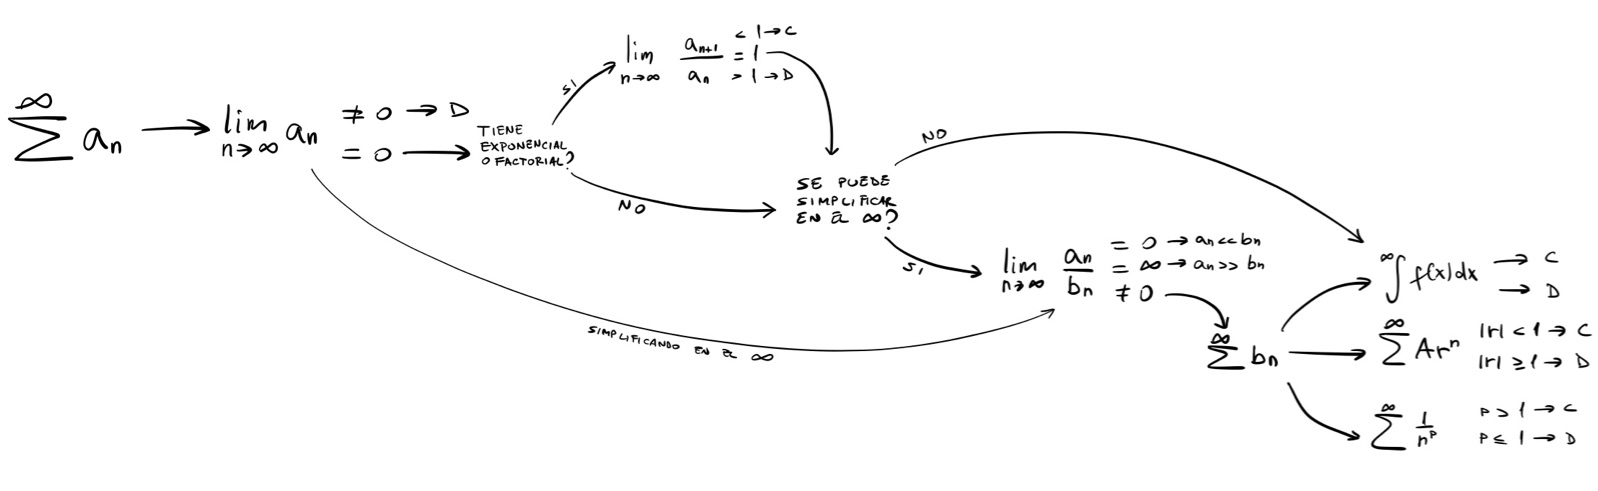
\includegraphics[width=12cm]{../../../../img/mapa_series}
\end{center}
\begin{enumerate}[a)]
\item $\sum\limits_{n=1}^{\infty}\dfrac{5n^3}{7n+n^3-1}$\\
			\\
			En primer lugar, veamos el límite de la sucesión, esto es
			$$\lim\limits_{n\ra \infty} \dfrac{5n^3}{7n+n^3-1} = 5 \neq 0$$
			Entonces, por la prueba de la divergencia, concluimos que la serie diverge.
\item $\sum\limits_{n=1}^{\infty}\left(sen\left(\dfrac{n\pi}{2}\right)\right)^2$\\
			\\
			Veamos el límite de la sucesión
			$$\lim\limits_{n\ra \infty} \left(sen\left(\dfrac{n\pi}{2}\right)\right)^2 \ra alternante \neq 0$$
			Por la prueba de la divergencia, la serie diverge.
\item $\sum\limits_{n=1}^{\infty}2^{2n}3^{1-3n}$\\
			\\
			Notemos que esta es una serie geométrica, por lo que debemos escribirla de la forma $\sum\limits_1^{\infty} Ar^n$ para saber como se comporta.
$$\sum\limits_{n=1}^{\infty}2^{2n}3^{1-3n} 
= \sum\limits_{n=1}^{\infty}2^{2n} \dfrac{3}{3^{3n}}
= \sum\limits_{n=1}^{\infty}(2^2)^n \dfrac{3}{(3^3)^n}
= \sum\limits_{n=1}^{\infty}4^n \dfrac{3}{27^n}
= \sum\limits_{n=1}^{\infty} 3 \left(\dfrac{4}{27}\right)^n$$
			Como $r = \dfrac{4}{27} <1$, la serie converge.
\item $\sum\limits_{n=1}^{\infty}\dfrac{1 + n + \sin(n)}{3n^4 + \ln(n)}$\\
			\\
En primer lugar, notemos que
$$\lim\limits_{n\ra \infty} \dfrac{1 + n + \sin(n)}{3n^4 + \ln(n)}
= \lim\limits_{n\ra \infty} \dfrac{n\left(\cancelto{0}{\frac{1}{n}} + 1 + \cancelto{0}{\frac{\sin(n)}{n}}\right)}{n^4\left(3 + \cancelto{0}{\frac{\ln(n)}{n^4}}\right)}
= \lim\limits_{n\ra \infty} \dfrac{n}{3n^4}
= \lim\limits_{n\ra \infty} \dfrac{1}{3n^3} = 0$$
Luego, usando $b_n = \dfrac{1}{3n^3}$, se cumple que
$$\lim\limits_{n\ra \infty} \dfrac{\dfrac{1 + n + \sin(n)}{3n^4 + \ln(n)}}{\dfrac{1}{3n^3}}
= \lim\limits_{n\ra \infty} \dfrac{\dfrac{1}{3n^3}}{\dfrac{1}{3n^3}} 
= 1 \neq 0$$
Notemos que $\sum\limits_{n=1}^{\infty} \dfrac{1}{3n^3}$ es es una $serie-p$ con $p=3>1$, por lo que la serie es convergente. Luego, por criterio de comparación al límite, $\sum\limits_{n=1}^{\infty}\dfrac{1 + n + \sin(n)}{3n^4 + \ln(n)}$ también converge.
\item $\sum\limits_{n=20}^{\infty}\dfrac{1}{nln(n)ln(ln(n))}$\\
			\\
			Sea
			$$a_n = \dfrac{1}{nln(n)ln(ln(n))} \ra f(x) = \dfrac{1}{xln(x)ln(ln(x))}$$
			Usando el criterio de la integral, $\displaystyle\int_{20}^{\infty}f(x)dx$ se comportará igual que $\sum\limits_{n=20}^{\infty} a_n$, por lo que debemos ver la convergencia de la integral en cuestión
			$$\int_{20}^{\infty} \dfrac{1}{xln(x)ln(ln(x))} dx$$
			Usando $u=ln(ln(x)) \ra du = \dfrac{dx}{xln(x)}$,
			$$\int_{20}^{\infty} \dfrac{1}{xln(x)ln(ln(x))} dx
			= \int_{ln(ln(20))}^{\infty} \dfrac{du}{u} = ln(u) \ev_{ln(ln(20))}^{\infty}$$
			$$ = ln(\infty) - ln(ln(ln(20))) = \infty = \not \exists$$
			Finalmente, por el criterio de la integral, la serie converge.
\item  $\sum\limits_{n=1}^{\infty}ln\left(1+\dfrac{1}{n}\right)$\\
			\\
			Notemos que
			$$\sum\limits_{n=1}^{\infty} ln\left(1+\dfrac{1}{n}\right)
			= \sum\limits_{n=1}^{\infty} ln\left(\dfrac{n+1}{n}\right)
			= \sum\limits_{n=1}^{\infty} ln(n+1)-ln(n)$$
			Es una serie telescopica. Expandiendo términos
			$$= (ln(2)-ln(1)) + (ln(3)-ln(2)) + \dots + (ln(n) - ln(n-1)) + (ln(n+1) - ln(n))$$
			$$= (\cancel{ln(2)}-ln(1)) + (\cancel{ln(3)}-\cancel{ln(2)}) + \cancel{\dots} + (\cancel{ln(n)} - \cancel{ln(n-1)}) + (ln(n+1) - \cancel{ln(n)})$$
			$$= ln(n+1) - ln(1)$$
			$$\lim\limits_{n \ra \infty} ln(n+1) = ln(\infty) = \infty = \not \exists$$
			Finalmente, la serie es divergente.
\end{enumerate}
\end{solucion}
\item Demuestre que si $\sum\limits_{n=1}^{\infty}a_n$ es convergente, entonces el limite de la sucesión $b_n=ln(1+a_n)$ en el infinito es $0$.
\begin{solucion}
Como $\sum\limits_{n=1}^{\infty}a_n$ es convergente, entonces debe ocurrir que
$\lim\limits_{x \ra \infty} a_n = 0$.\\

Luego,
$$\lim\limits_{x \ra \infty} b_n
= \lim\limits_{x \ra \infty} ln(1+a_n)
= ln(1+\lim\limits_{x \ra \infty} a_n)
= ln(1+0)
= 0$$

$$\blacksquare$$
\end{solucion}
\item Sea $a_n$ una sucesión tal que $a_n \neq 0,\ \forall n \in \N$.\\
	Demuestre que si $\sum\limits_{n=1}^{\infty}a_n$ converge, entonces $\sum\limits_{n=1}^{\infty}\dfrac{1}{a_n}$ diverge.
\begin{solucion}
Como $\sum\limits_{n=1}^{\infty}a_n$ es convergente, entonces debe ocurrir que
$\lim\limits_{x \ra \infty} a_n = 0$.\\

Luego,
$$\lim\limits_{x \ra \infty} \dfrac{1}{a_n}
= \dfrac{1}{\lim\limits_{x \ra \infty} a_n}
= \dfrac{1}{0}
= \infty
\neq 0$$
Entonces, por la prueba de la divergencia, $\sum\limits_{n=1}^{\infty}\dfrac{1}{a_n}$ diverge.
\end{solucion}
\item Considere una función $f$ continua en $\R$, decreciente y no negativa tal que
	$$\lim_{x\ra\infty}\dfrac{f(x)}{e^{-x}}=5$$
	Analice la convergencia de la serie $\sum\limits_{n=1}^{\infty}f(n)$
\begin{solucion}
Sabemos que
		$$\lim_{x\ra\infty}\dfrac{f(x)}{e^{-x}}=5 \neq 0$$
		Por lo tanto, por el criterio de comparación al límite, $\sum\limits_{n=1}^{\infty}f(n)$ se comporta igual que $\sum\limits_{n=1}^{\infty}e^{-n}$\\
		\\
		Veamos la convergencia de 
		$$\sum\limits_{n=1}^{\infty}e^{-n}$$
		Usando el criterio de la razón,
		$$\lim\limits_{n \ra \infty} \dfrac{a_{n+1}}{a_n}
		= \lim\limits_{n \ra \infty} \dfrac{e^{-n-1}}{e^{-n}}
		= e^{-1} < 1$$
		Por lo tanto, es convergente. De la misma forma, la serie $\sum\limits_{n=1}^{\infty}f(n)$ también lo es.
\\
\\
Otra forma de determinar la convergencia es notando que esta es una serie geométrica con $r = \dfrac{1}{e} < 1$.
\end{solucion}
\item Considere la representación decimal de un número,
$$0,d_1d_2d_3... = \dfrac{d_1}{10} + \dfrac{d_2}{10^2} + \dfrac{d_3}{10^3}$$
donde $d_i$ es alguno de los dígitos entre 0 y 9. Pruebe que la serie anterior es convergente.
\begin{solucion}
Del enunciado, podemos ver que esta serie se puede escribir como
$$\sum\limits_{1}^{\infty} \dfrac{d_n}{10^n}$$
Notemos que el valor máximo que tomara cualquier $d_n$ es 9, por lo que podemos encontrar una serie que acote superiormente a esta simplemente reemplazando $d_n$ con 10, es decir
$$\sum\limits_{1}^{\infty} \dfrac{d_n}{10^n} < \sum\limits_{1}^{\infty} \dfrac{10}{10^n}$$
Notemos que esta última corresponde a la serie geométrica
$$\sum\limits_{1}^{\infty} 10\left(\dfrac{1}{10}\right)^n$$
La cual es convergente, dado que $r = \dfrac{1}{10} < 1$.
Por último, por criterio de comparación simple, concluimos que la serie pedida también converge.
\end{solucion}
\end{preguntas}
\end{document}